% !TEX program = xelatex
\documentclass{article}

\title{Notite examen - Sisteme de Operare}
\date{}
\author{Dinu Florin-Silviu \\ grupa 231}

\newcommand{\prim}{^\ensuremath{\prime}}
\newcommand{\secund}{^{\ensuremath{\prime\prime}}}

% \makeatletter
% \renewcommand{\@seccntformat}[1]{}
% \makeatother

\newenvironment{textColor}[1]{%
    \leavevmode\color{#1}\ignorespaces%
}{%
}%


\usepackage{tikz}
\usepackage{forest}
\usepackage{hyperref}
\usepackage{amsthm}
\usepackage{amssymb}
\usepackage[english]{babel}
\usepackage[a4paper, margin=3cm]{geometry}
\usepackage{enumitem}
\usepackage{listings}
\usepackage{fontspec}
\usepackage{xcolor}
\usepackage{textcomp}
\usepackage{graphicx}
\usepackage{tabularx}
\usepackage{pgfgantt}

\graphicspath{ {./img/} }

\newfontfamily{\ttconsolas}{Consolas}
\lstset{
%  tabsize=4,
extendedchars=true,
        basicstyle=\ttconsolas,
        % %upquote=false,
        % aboveskip=\baselineskip,
        columns=fixed,
        showstringspaces=false,
        extendedchars=true,
        breaklines=true,
        % prebreak = \raisebox{0ex}[0ex][0ex]{\ensuremath{\hookleftarrow}},
        showtabs=false,
        showspaces=false,
        identifierstyle=\ttfamily,
        % keywordstyle=\color[rgb]{0,0,1},
        % commentstyle=\color[rgb]{0.133,0.545,0.133},
        % stringstyle=\color[rgb]{0.627,0.126,0.941},
        % language=SQL
        frame=lines,
        literate=%
    {€}{\euro}1%
    {§}{\S}1%
    {°}{\textdegree{}}1%
    {ä}{{\"a}}1%
    {ö}{{\"o}}1%
    {ü}{{\"u}}1%
    {ß}{{\ss}}1%
    {Ä}{{\"A}}1%
    {Ö}{{\"O}}1%
    {Ü}{{\"U}}1%
    {µ}{\textmu}1%
    {¹}{{\textsuperscript{1}}}1%
    {²}{{\textsuperscript{2}}}1%
    {³}{{\textsuperscript{3}}}1%
    {¼}{\textonequarter}1%
    {½}{\textonehalf}1%
    {¢}{\textcent}1%
}


\tikzstyle{red state}=[
        draw = red,
        thick,
        fill = white,
        minimum size = 4mm,
        circle
    ]

\tikzstyle{blue state}=[
    draw = blue,
    thick,
    fill = white,
    minimum size = 4mm,
    circle
]

\tikzstyle{green state}=[
    draw = green,
    thick,
    fill = white,
    minimum size = 4mm,
    circle
]

\tikzset{
  gray box/.style={
    fill=gray!20,
    draw=gray,
    minimum width={1.5*#1ex},
    minimum height={2em},
  },
  annotation/.style={
    anchor=north,
  }
}

\newtheorem*{theorem}{Teorema}
\renewcommand\qedsymbol{QED}

\begin{document}
\pagenumbering{gobble}
\maketitle
\tableofcontents

\newpage
\pagenumbering{arabic}

\section[Ch3 Processes]{Processes}
\subsection*{States}
\begin{enumerate}
    \item New - e creat
    \item Running - se executa instructiunile
    \item Waiting - asteapta un eveniment
    \item Ready - asteapta sa fie asignat unui procesor
    \item Terminated - a terminat executia
\end{enumerate}

\begin{center}
    \includegraphics[scale=0.4]{1_procese.png}
\end{center}

\subsection*{Task control block}
\begin{enumerate}
    \item Process state
    \item Program counter (location of next instruction)
    \item CPU registers (contents of all process-centric registers)
    \item CPU scheduling information (priorities, scheduling queue pointers)
    \item Memory-management information (memory allocated to the process)
    \item Accounting information (CPU used, clock time since start, time limits)
    \item I/O status information (I/O devices allocated to the process, list of open files)
\end{enumerate}

\begin{center}
    \includegraphics[scale=0.3]{2_taskcontrolblock.png}
\end{center}

\subsection*{Process scheduling}
\paragraph*{Process scheduler} selects among available processes for next execution on CPU core
\subparagraph*{Goal} - maximize CPU use, quickly switch processes onto CPU core
\subparagraph*{Scheduling queues} Ready queue and wait queue

\begin{center}
    \includegraphics[scale=0.3]{3_processqueue.png}
\end{center}

\begin{center}
    \includegraphics[scale=0.3]{4_indepthprocsched.png}
\end{center}

\subsection*{Context switch} Ehen CPU switches to another process, the system must save the state of the old process and load the save state for the new process via a context switch
\paragraph*{Contextul} unui proces este reprezentat in PCB

\subsection*{Process creation}
\paragraph*{Parintii} creaza copii care, la randul lor, pot crea alte procese, formand un arbore de procese
\subparagraph*{PID} - process identifier ID
\paragraph*{Partajarea de resurse - optiuni}
\begin{enumerate}
    \item Parintii si copiii partajeaza toate resursele
    \item Copiii folosesc o submultime a resurselor parintilor
    \item Parintii si copiii nu partajeaza nicio resursa
\end{enumerate}
\paragraph*{Executie - optiuni}
\begin{enumerate}
    \item Parintii si copiii se executa concurent
    \item Parintele asteapta sa termine copilul
\end{enumerate}

\paragraph*{Spatiu de adresa}
\begin{enumerate}
    \item Copilul e un duplicat al parintelui
    \item Copilul are un program incarcat in el
\end{enumerate}

\paragraph*{Exemple UNIX}
\begin{enumerate}
    \item fork() - syscall pentru crearea de noi procese
    \item exec() - syscall dupa fork() ca sa inlocuiasca memory space-ul cu un alt program
    \item wait() - parintele asteapta sa termine copilul
\end{enumerate}

\subsection*{Process termination}
\paragraph*{exit()} - procesele executa ca ultima instructiune syscallul exit() care returneaza statusul catre parinte via wait() si resursele sunt dealocate de sistem
\paragraph*{abort()} - parintele poate termina oricand copilul. Unele din motive sunt: copilul a depasit resursele alocate, ceea ce i s-a cerut copilului nu mai este necesar, parintele a apelat exit() si sistemul nu mai lasa copilul sa continue in acest caz (terminarea in cascada)
\paragraph*{Zombie} nu mai are parinte care sa astepte (nu s-a invocat wait())
\paragraph*{Orfan} parintele s-a terminat fara sa invoce wait()

\subsection*{Interprocess Communication}
\paragraph*{Procesele} pot fi independente sau sa coopereze
\subparagraph*{Cooperarea} inseamna ca procesul poate fi afectate sau afecta alte procese, inclusiv datele partajate
\paragraph*{Motive pentru cooperare}
\begin{enumerate}
    \item Partajarea de informatie
    \item Viteza de calcul mai mare
    \item Modularitate
    \item Convenienta
\end{enumerate}
\paragraph*{IPC - 2 modele}
\begin{enumerate}
    \item memorie partajata
    \item pasare de mesaje
\end{enumerate}

\begin{center}
    \includegraphics[scale=0.3]{5_ipc.png}
\end{center}

\subsection*{Shared memory}

\paragraph*{Producer-consumer}: producatorul produce informatie care e consumata de consumator
\subparagraph*{2 variante}
\begin{enumerate}
    \item unbounded-buffer - nu are limite practice asupra marimii bufferului
    \begin{enumerate}
        \item producatorul nu asteapta
        \item consumatorul asteapta daca nu e buffer de consumat
    \end{enumerate}
    \item bounded-buffer - toate bufferele au marime fixa
    \begin{enumerate}
        \item producatorul trebuie sa astepte daca toate bufferele sunt full
        \item consumatorul asteapta daca nu e buffer pe care sa-l consume
    \end{enumerate}
\end{enumerate}

\paragraph*{Umplerea TUTUROR bufferelor} se face cu un counter care e 0, e incrementat de producator cu fiecare buffer si decrementat de consumator dupa ce il consuma

\paragraph*{Race condition}

\begin{center}
    \includegraphics[scale=0.3]{6_racecondition.png}
\end{center}


\subsection*{Message passing}
\paragraph*{2 operatii}: send(message), receive(message)
\paragraph*{Communication link}
\begin{enumerate}
    \item Physical
    \begin{enumerate}
        \item Shared memory
        \item Hardware bus
        \item Network
    \end{enumerate}
    \item Logical
    \begin{enumerate}
        \item Direct sau indirect
        \item Sincron sau asincron
        \item Buffering automat sau explicit
    \end{enumerate}
\end{enumerate}

\paragraph*{Comunicarea directa}
\subparagraph*{Se denumesc explicit} send(P, msg) sau receive(Q, msg)
\subparagraph*{Avantaje}
\begin{enumerate}
    \item Linkurile sunt stabilite automat
    \item Linkurile sunt asociate cu exact o pereche de procese care comunica
    \item Intre 2 procese este exact 1 link
    \item Linkul poate fi unidrectional, dar de obicei, e bidirectional
\end{enumerate}

\paragraph*{Comunicarea indirecta}
\subparagraph*{Mesajele vin din mailboxes (ports)} Fiecare mailbox are ID unic, procesele pot comunica doar daca partajeaza un mailbox
\subparagraph*{Proprietatile linkului de comunicare}
\begin{enumerate}
    \item Linkurile sunt stabilite doar daca e un mailbox comun
    \item Un link poate fi asociat cu mai multe procese
    \item Perechile de procese pot avea in comun mai multe linkuri
    \item Linkul poate fi unidirectional sau bidirectional
\end{enumerate}
\subparagraph*{Operatii}
\begin{enumerate}
    \item Crearea de mailbox (port)
    \item Send and receive
    \item Delete
\end{enumerate}
\subparagraph*{Primitive} send(A, msg), receive(A, msg)

\paragraph*{Pasarea de mesaje}
\begin{enumerate}
    \item Blocking
    \begin{enumerate}
        \item Blocking send
        \item Blocking receive
    \end{enumerate}
    \item Non-blocking
    \begin{enumerate}
        \item Non-blocking send
        \item Non-blocking receive
    \end{enumerate}
    \item Alte combinatii: daca avem send si receive blocking, avem \textbf{rendezvous}
\end{enumerate}

\paragraph*{Buffering}
\subparagraph*{Queue} atasata unui link
\subparagraph*{3 implementari:}
\begin{enumerate}
    \item Zero capcity - fara mesaje pe link. Senderul asteapta pentru receiver (rendezvous)
    \item Bounded capacity - lungime finita de n mesaje. Senderul asteapta daca linkul e full
    \item Unbounded capacity - lungime infinita. Senderul nu asteapta niciodata
\end{enumerate}

\begin{center}
    \includegraphics[scale=0.3]{7_sharedmem.png}
\end{center}

\subsection*{Mach}
\paragraph*{Message based}
\begin{enumerate}
    \item syscallurile sunt mesaje
    \item toate taskurile au 2 porturi la creare: kernel si notify
    \item mesajele sunt trimise si primite cu mach\_msg()
    \item portul e creat cu mach\_port\_allocate()
    \item send si receive sunt flexibile, 4 optiuni daca mailboxul e full
    \begin{enumerate}
        \item asteapta nedefinit
        \item asteapta max n ms
        \item returneaza imediat
        \item cachuieste un mesaj temporar
    \end{enumerate}
\end{enumerate}

\subsection*{Pipes}
\paragraph*{Comunicare intre 2 procese}
\subsection*{Ordinary pipes}
\paragraph*{Nu pot fi accesate din afara procesului care le-a creat}
\begin{enumerate}
    \item Comunicare standard in stil producer-consumer
    \item Producerul: write-end of the pipe
    \item Consumerul: read-end of the pipe
    \item Unidirectionale
    \item Au nevoie de parent-child
\end{enumerate}

\subsection*{Named pipes}
\paragraph*{Pot fi accesate fara relatie parent-child}
\begin{enumerate}
    \item Comunicarea e bidirectionoala
    \item Nu e nevoie de parent-child
    \item Mai multe procese pot folosi acelasi pipe
\end{enumerate}

\subsection*{Sistemele client-server}
\paragraph*{Sockets}
\begin{enumerate}
    \item endpoint de comunicare
    \item IP:PORT
    \item <1024 well known
    \item 127.0.0.1 loopback
\end{enumerate}
\paragraph*{RPC}
\begin{enumerate}
    \item Abstractizeaza procedura callurilor dintre procese si sistemele din retea
    \item foloseste porturi
    \item stubs - client-side proxy pentru procedura actuala din server
    \item stubul localizeaza serverul si marshalls parametrii
    \item server-side stub primeste mesajul, dezpacheteaza parametrii si face procedura
    \item reprezentarea datelor se face prin XDL (External Data Representation)
    \item comunicarea are mai multe failure scenarios (mesajele pot fi trimise o SINGURA data sau CEL MULT o data)
    \item OS-ul are un rendezvous (sau matchmaker) service ca sa conecteze clientul si serverul
\end{enumerate}

\section[Ch4 Threads and Concurrency]{Threads and Concurrency}
\paragraph*{Beneficii}
\begin{enumerate}
    \item Responsivness - continuarea executiei daca o parte din proces e blocata (UI)
    \item Resource Sharing - partajeaza cu procesele mai usor ca shared memory sau message passing
    \item Economie - mai ieftin decat crearea proceselor, iar threa switching mai ieftin ca message passing
    \item Scalabilitate - procesele pot folosi arhitecturile multicore
\end{enumerate}

\paragraph*{Paralelism} - un sistem poate face mai mult de 1 lucru simultan
\paragraph*{Concurrency} - sustine mai mult de un task care face progres (single processor/core - scheduler providing concurrency)

\paragraph*{Tipuri de paralelism}
\begin{enumerate}
    \item Data paralelism - distribuie submultimi ale datelor pe mai multe coreuri, aceeasi operatie pentru fiecare
    \item Task parallelism - distribuie threadurile pe coreuri, fiecare thread facand o actiune unica
\end{enumerate}

\paragraph*{Legea lui Amdahl}

\begin{center}
    \begin{math}
        speedup \leq \frac{1}{S+\frac{(1-S)}{N}}
    \end{math}
\end{center}

\subparagraph*{title} S = portiunea seriala, N = numarul de coreuri

\paragraph*{User vs Kernel Threads}

\subsection*{Modele multithreading}
\begin{enumerate}
    \item Many-to-One
    \item One-to-One
    \item Many-to-Many
\end{enumerate}

\paragraph*{Many-to-one}
\begin{enumerate}
    \item Mai multe threaduri user-level mapate pe un thread de kernel
    \item Un thread blocking le face pe toate sa se blocheze
    \item Mai multe threaduri pot sa nu ruleze in paralel pe un sistem multicore pentru ca numai unul poate fi in kernel la un moment dat
    \item Exemple: Solaris Green Threads, GNU Portable Threads
\end{enumerate}
\paragraph*{One-to-One}
\begin{enumerate}
    \item Fiecare thread user-level mapeaza pe un thread al kernelului
    \item Crearea unui thread la user level creaza un thread in kernel
    \item Mai multa concurenta decat many-to-one
    \item Numarul de threaduri pe proces restrictionat din cauza overheadului
\end{enumerate}
\paragraph*{Many-to-Many}
\begin{enumerate}
    \item Mai multe user level threads mapate pe mai multe kernel threads
    \item Sistemul poate crea un numar suficient de threaduri de kernel
    \item Exemplu (necomun): ThreadFiber pe Windows
\end{enumerate}
\paragraph*{Two-level Model} Ca M:M, doar ca un user thread poate fi bound catre un kernel thread

\begin{center}
    \includegraphics[scale=0.3]{8_twolevelmodel.png}
\end{center}

\subsection*{Pthreads}
\begin{enumerate}
    \item User-level sau kernel-level
    \item Un API POSIX standard pentru crearea si sincronizarea threadurilor
    \item Specificatie, nu implementare
    \item API-ul specifica comportamentul librariei, nu al implementarii
    \item Comun in UNIX 
\end{enumerate}

\subsection*{Implicit threading}
\begin{enumerate}
    \item Thread Pools
    \item Fork-Join
    \item OpenMP
    \item Grand Central Dispatch
    \item Intel Threading BUilding Blocks
\end{enumerate}

\paragraph*{Thread Pools} Creaza un numar de threaduri intr-o piscina unde asteapta munca
\begin{enumerate}
    \item De obicei ceva mai rapide sa preia un request cu unul existent decat cu crearea unuia nou
    \item Nr de threaduri maxim marimea poolului
    \item Separarea taskurilor de mecanismele de creare a taskurilor permit diferite strategii de run (ex: periodical schedule)
\end{enumerate}

\paragraph*{Fork-join Parallelism} Mai mult threaduri sunt forkuite, apoi joinate

\begin{center}
    \includegraphics[scale=0.3]{9_forkjoin.png}
\end{center}

\subparagraph*{Algoritmul general}
\begin{center}
    \begin{lstlisting}
Task(problem){
    if (problem is small enough){
        solve directly;
    } else {
        subtask1 = fork (new Task (subset of problem));
        subtask2 = fork (new Task (subset of problem));

        result1 = join(subtask1);
        result2 = join(subtask2);

        return combined results;
    }
}
    \end{lstlisting}
\end{center}

\begin{center}
    \includegraphics[scale=0.3]{10_forkjoin.png}
\end{center}

\paragraph*{OpenMP}
\begin{enumerate}
    \item O multime de directive de compilator si un API pentru C, C++, FROTRAN
    \item Suport pentru programarea paralela in mediile cu shared-memory
    \item Identifica regiunile paralele (blocheaza codul paralel)
    \item Se creaza threaduri pe cat de multe coreuri sunt
\end{enumerate}

\paragraph*{Grand Central Dispatch}
\begin{enumerate}
    \item Apple technology for macOS and iOS
    \item Extensii C, C++ si Objective-C, API si librarie run-time
    \item Permite identificarea sectiunilor paralele
    \item Gestioneaza majoritatea detaliilor in threading
    \item Blocul este intre \^\ \{\}
    \item Blocurile sunt puse in dispatch queue si sunt asignate unui thread disponibil din pool cand sunt scoase din coada
    \item Doua tipuri de dispatch queues
    \begin{enumerate}
        \item serial - FIFO, queue per proces, numit main queue
        \item concurent - FIFO, dar mai multe o data
    \end{enumerate}
\end{enumerate}

\subsection*{Threading issues}
\paragraph*{Semantica fork() si exec()}
\subparagraph*{Fork()} de obicei duplica doar calling thread (Linux), dar pe alte sisteme, toate threadurile
\subparagraph*{Exec()} de obicei inlocuieste procesul care ruleaza inclusiv threadurile sale

\paragraph*{Signal handling} folosit pentru procesarea semnalelor
\begin{enumerate}
    \item Semnal generat de un anumit eveniment
    \item Semnalul este dat unui proces
    \item Semnalul este ahndeluit de 1 din cele doua handleluri
    \begin{enumerate}
        \item default
        \item user-defined
    \end{enumerate}
\end{enumerate}

\paragraph*{Thread Cancellation} Terminarea unui thread (numit si target thread) inainte de sfarsit
\subparagraph*{2 metode:} Asincrona (imediata), Deferred (target threadul verifica periodic daca trebuie cancelat). Tipul implicit e deferred. Pe Linux thread cancellation e obtinut prin semnale

\paragraph*{TLS (Thread Local Storage)} permite fiecarui thread sa aiba copia proprie a datelor si e folositor la thread pooluri (unde nu ai control asupra crearii)

\subsection*{Scheduler Activations}
M:M si Two-level au nevoie de comunicare pentru a aloca numarul potrivit de threaduri de Kernel. De obicei se foloseste o structura de date intermediara intre threadurile de user si de kernel LWP (lightweight process). Acesta apare ca un procesor virtual unde procesele pot face scheduleing pentru rularea user threadurilor, fiecare LWP e atasat unui thread de kernel. Scheduler activations au upcalls (un mecanism de comunicare de la kernel la upcall handler)

\subsection*{Linux threads}
\begin{enumerate}
    \item Li se zice tasks
    \item Se fac prin syscallul clone()
    \item clone() permite taskurilor copil sa partajeze address space-ul parintelui (procesului)
\end{enumerate}

\section[Ch5 CPU Scheduling]{CPU Scheduling}
\paragraph*{CPU - I/O Burst cycle} un ciclu de cpu execution si I/O wait

\begin{center}
    \includegraphics[scale=0.3]{11_cpuioburstcycle.png}
\end{center}

\subsection*{CPU Scheduler} Selecteaza din procesele din queue (ordonata in moduri diferite) si aloca un core de CPU unuia
\subparagraph*{Deciziile pot avea loc atunci cand:}
\begin{enumerate}
    \item Running $\rightarrow$ waiting
    \item Running $\rightarrow$ ready
    \item Waiting $\rightarrow$ ready
    \item Terminates
\end{enumerate}
\subparagraph*{Optiuni:} Pentru 1 \& 4 \textbf{NU} exista, pentru 2 \& 3 exista. Asadar pentru 1 \& 4 este nonpreemptive (o data alocat, procesul pastreaza CPU-ul pana se termina sau se schimba la waiting), altfel este preemptive. 
\subparagraph*{Preemptive} poate duce la race conditions

\subsection*{Dispatcher}
\paragraph*{Dispatcher-ul} da controlul CPU-ului procesului selectat de \textbf{scheduler}. Acest lucru inseamna: schimbarea de context, schimbarea in user mode, jump la locatia din programul userului pentru a restarta programul
\paragraph*{Dispatch latency} - timpul care ii ia dispatcher-ului sa opreasca un proces, apoi sa ruleze altul

\subsection*{Scheduling criteria}
\begin{enumerate}
    \item \textbf{CPU utilizations} - sa fie cat mai ocupat
    \item \textbf{Throughput} - nr de procese care isi completeaza executia per unitate de timp
    \item \textbf{Turnaround time} - timpul de executie al unui proces
    \item \textbf{Waiting time} - timpul pe care un proces l-a petrecut in ready queue
    \item \textbf{Response time} - timpul pe care un proces il petrece de cand a facut o cerere pana cand primul raspuns este produs
\end{enumerate}

\subsection*{FCFS (First-Come, First-Served)}
\paragraph*{Convoy effect} - short process behind long process
\begin{center}
    \begin{tabularx}{0.8\textwidth} {
            | >{\centering\arraybackslash}X
            | >{\centering\arraybackslash}X
            |}
        \hline
          Process & Burst Time \\
        \hline
        $P_1$ & 24 \\
        $P_2$ & 3 \\
        $P_3$ & 3 \\
        \hline
    \end{tabularx}
\end{center}

\begin{center}
    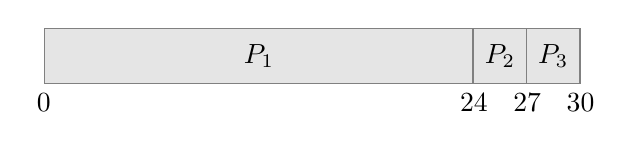
\begin{tikzpicture}[node distance=-0.5pt]
        \node [gray box=24] (p1) {\(P_{1}\)};
        \node [gray box=3, right=of p1] (p2) {\(P_{2}\)};
        \node [gray box=3, right=of p2] (p3) {\(P_{3}\)};
      
        \node [annotation] at (p1.south west) {0};
        \node [annotation] at (p1.south east) {24};
        \node [annotation] at (p2.south east) {27};
        \node [annotation] at (p3.south east) {30};
    \end{tikzpicture}
\end{center}
\paragraph*{Waiting time:} $P_1 = 0$; $P_2 = 24$; $P_3 = 27$
\paragraph*{Average waiting time:} $\frac{(0+24+27)}{3} = 17$

\subsection*{SJF (Shortest-Job-First)}
\paragraph*{SJF e optim} - are media timpurilor de asteptare pentru o multime de procese ca fiind minima
\paragraph*{Shortest-remaining-time-first} este numele versiunii preemptive

\begin{center}
    \begin{tabularx}{0.8\textwidth} {
            | >{\centering\arraybackslash}X
            | >{\centering\arraybackslash}X
            |}
        \hline
          Process & Burst Time \\
        \hline
        $P_1$ & 6 \\
        $P_2$ & 8 \\
        $P_3$ & 7 \\
        $P_4$ & 3 \\
        \hline
    \end{tabularx}
\end{center}

\begin{center}
    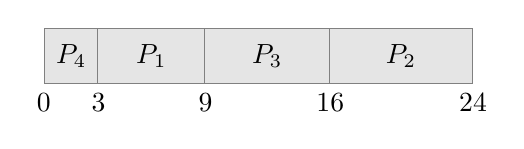
\begin{tikzpicture}[node distance=-0.5pt]
        \node [gray box=3] (p4) {\(P_{4}\)};
        \node [gray box=6, right=of p4] (p1) {\(P_{1}\)};
        \node [gray box=7, right=of p1] (p3) {\(P_{3}\)};
        \node [gray box=8, right=of p3] (p2) {\(P_{2}\)};
      
        \node [annotation] at (p4.south west) {0};
        \node [annotation] at (p4.south east) {3};
        \node [annotation] at (p1.south east) {9};
        \node [annotation] at (p3.south east) {16};
        \node [annotation] at (p2.south east) {24};
    \end{tikzpicture}
\end{center}

\paragraph*{Average waiting time:} $\frac{(3+16+9+0)}{4} = 7$

\paragraph*{Cum determinam lungimea CPU burst?} 
\subparagraph*{Estimare:} ar trebui sa fie asemanatoare cu cele anterioare. Poate fi folosita cu exponential averaging
\begin{enumerate}
    \item $t_n$ = lungimea reala a celui de-al n-ulea CPU burst
    \item $\tau_{n+1}$ = valoarea prezisa pentru urmatorul CPU burst
    \item $\alpha,0 \leq \alpha \leq 1$ (de obicei e setat la $\frac{1}{2}$)
    \item Definim: $\tau_{n+1} = \alpha t_n + (1-\alpha) \tau_{n}$
\end{enumerate}

\subsection*{Shortest Remaning Time First}
\paragraph*{SJN} - versiunea preemtiva. Cand ajunge in coada de ready, decizia de a-l programa urmatorul este refacuta cu alogirtmul SJN

\begin{center}
    \begin{tabularx}{0.8\textwidth} {
            | >{\centering\arraybackslash}X
            | >{\centering\arraybackslash}X
            | >{\centering\arraybackslash}X
            |}
        \hline
          Process & Arrival Time & Burst Time \\
        \hline
        $P_1$ & 0 & 8 \\
        $P_2$ & 1 & 4 \\
        $P_3$ & 2 & 9 \\
        $P_4$ & 3 & 5 \\
        \hline
    \end{tabularx}
\end{center}

\begin{center}
    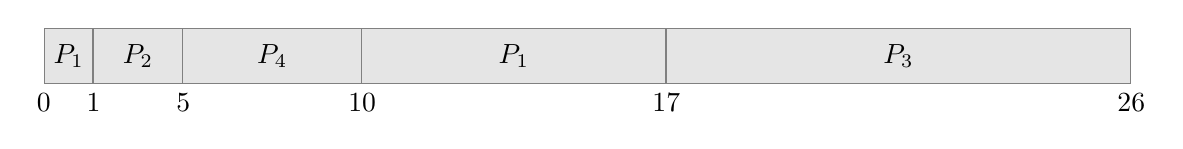
\begin{tikzpicture}[node distance=-0.3pt]
        \node [gray box=1] (p1) {\(P_{1}\)};
        \node [gray box=5, right=of p1] (p2) {\(P_{2}\)};
        \node [gray box=10, right=of p2] (p4) {\(P_{4}\)};
        \node [gray box=17, right=of p4] (p11) {\(P_{1}\)};
        \node [gray box=26, right=of p11] (p3) {\(P_{3}\)};
      
        \node [annotation] at (p1.south west) {0};
        \node [annotation] at (p1.south east) {1};
        \node [annotation] at (p2.south east) {5};
        \node [annotation] at (p4.south east) {10};
        \node [annotation] at (p11.south east) {17};
        \node [annotation] at (p3.south east) {26};
    \end{tikzpicture}
\end{center}

\begin{center}
    \begin{tabularx}{0.8\textwidth} {
            | >{\centering\arraybackslash}X
            | >{\centering\arraybackslash}X
            | >{\centering\arraybackslash}X
            | >{\centering\arraybackslash}X
            |}
        \hline
          Process & Completion Time & Turnaround Time (CT-AT) & Waiting time (TAT-BT) \\
        \hline
        $P_1$ & 17 & 17 & 9 \\
        $P_2$ & 5 & 4 & 0\\
        $P_3$ & 26 & 24 & 15\\
        $P_4$ & 10 & 7 & 2\\
        \hline
    \end{tabularx}
\end{center}

\paragraph*{Average waiting time:} $[9+0+15+2]/4 = 26/4 = 6.5$

\subsection*{Round Robin (RR)}
\begin{enumerate}
    \item Fiecare proces ia o unitate mica de timp pe CPU (\textbf{time quantum} $q$), de obicei intre 10-100 ms. Dupa aceast timp, procesul este preempted si adaugat la sfarsitul queueului de ready
    \item Daca sunt n procese si time quantum este q, atunci ficare proces ia bucati de $\frac{1}{n}$ din timpul CPU-ului de cel mult q unitati de timp o data. Niciun proces nu asteapta mai mult de $(n-1)q$ unitati de timp
    \item Exista un timer care intrerupe fiecare quantum pentru scheduleing pe noul proces
    \item Performanta:
    \begin{enumerate}
        \item q mare $\approx$ FIFO(FCFS)
        \item q mic $\approx$ RR
    \end{enumerate}
\end{enumerate}

\begin{center}
    \begin{tabularx}{0.8\textwidth} {
            | >{\centering\arraybackslash}X
            | >{\centering\arraybackslash}X
            |}
        \hline
          Process & Burst Time \\
        \hline
        $P_1$ & 24 \\
        $P_2$ & 3\\
        $P_3$ & 3\\
        \hline
    \end{tabularx}
\end{center}

\begin{center}
    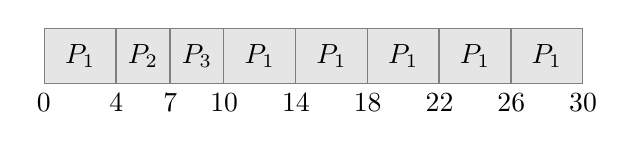
\begin{tikzpicture}[node distance=-0.3pt]
        \node [gray box=4] (p1) {\(P_{1}\)};
        \node [gray box=3, right=of p1] (p2) {\(P_{2}\)};
        \node [gray box=3, right=of p2] (p3) {\(P_{3}\)};
        \node [gray box=4, right=of p3] (p11) {\(P_{1}\)};
        \node [gray box=4, right=of p11] (p112) {\(P_{1}\)};
        \node [gray box=4, right=of p112] (p111) {\(P_{1}\)};
        \node [gray box=4, right=of p111] (p1111) {\(P_{1}\)};
        \node [gray box=4, right=of p1111] (p11111) {\(P_{1}\)};
      
        \node [annotation] at (p1.south west) {0};
        \node [annotation] at (p1.south east) {4};
        \node [annotation] at (p2.south east) {7};
        \node [annotation] at (p3.south east) {10};
        \node [annotation] at (p11.south east) {14};
        \node [annotation] at (p112.south east) {18};
        \node [annotation] at (p111.south east) {22};
        \node [annotation] at (p1111.south east) {26};
        \node [annotation] at (p11111.south east) {30};
    \end{tikzpicture}
\end{center}
\begin{center}
    \textbf{A fost folosit time quantum = 4}
\end{center}

\paragraph*{De obicei $TAT \ge SJF$, dar raspuns mai bun}
\paragraph*{q trebuie sa fie mai mare decat timpul de context switch.} De obicei q intre 10ms si 100ms, iar context switch $\le 10 \mu s$

\subsection*{Priority Scheduling}
\paragraph*{Priority number} - integer asociat fiecarui proces (nr mic - prioritate mare)
\paragraph*{SJF} este un priority scheduling unde prioritatea este inversul timpului urmator de CPU burst prezis
\paragraph*{Problema} Starvation $\Rightarrow$ \textbf{Solutie} Aging

\begin{center}
    \begin{tabularx}{0.8\textwidth} {
            | >{\centering\arraybackslash}X
            | >{\centering\arraybackslash}X
            | >{\centering\arraybackslash}X
            |}
        \hline
          Process & Burst Time & Priority \\
        \hline
        $P_1$ & 10 & 3 \\
        $P_2$ & 1 & 1 \\
        $P_3$ & 2 & 4 \\
        $P_4$ & 1 & 5 \\
        $P_5$ & 5 & 2 \\
        \hline
    \end{tabularx}
\end{center}

\begin{center}
    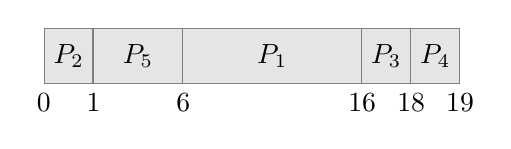
\begin{tikzpicture}[node distance=-0.3pt]
        \node [gray box=1] (p2) {\(P_{2}\)};
        \node [gray box=5, right=of p2] (p5) {\(P_{5}\)};
        \node [gray box=10, right=of p5] (p1) {\(P_{1}\)};
        \node [gray box=2, right=of p1] (p3) {\(P_{3}\)};
        \node [gray box=1, right=of p3] (p4) {\(P_{4}\)};
      
        \node [annotation] at (p2.south west) {0};
        \node [annotation] at (p2.south east) {1};
        \node [annotation] at (p5.south east) {6};
        \node [annotation] at (p1.south east) {16};
        \node [annotation] at (p3.south east) {18};
        \node [annotation] at (p4.south east) {19};
    \end{tikzpicture}
\end{center}

\paragraph*{Priority Scheduling cu Round-Robin (time quantum = 2)}
\begin{center}
    \begin{tabularx}{0.8\textwidth} {
            | >{\centering\arraybackslash}X
            | >{\centering\arraybackslash}X
            | >{\centering\arraybackslash}X
            |}
        \hline
          Process & Burst Time & Priority \\
        \hline
        $P_1$ & 4 & 3 \\
        $P_2$ & 5 & 2 \\
        $P_3$ & 8 & 2 \\
        $P_4$ & 7 & 1 \\
        $P_5$ & 3 & 3 \\
        \hline
    \end{tabularx}
\end{center}

\begin{center}
    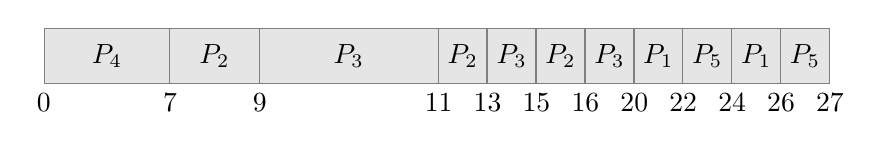
\begin{tikzpicture}[node distance=-0.3pt]
        \node [gray box=7] (p4) {\(P_{4}\)};
        \node [gray box=5, right=of p4] (p2) {\(P_{2}\)};
        \node [gray box=10, right=of p2] (p3) {\(P_{3}\)};
        \node [gray box=2, right=of p3] (p2i) {\(P_{2}\)};
        \node [gray box=1, right=of p2i] (p3i) {\(P_{3}\)};
        \node [gray box=1, right=of p3i] (p2ii) {\(P_{2}\)};
        \node [gray box=1, right=of p2ii] (p3ii) {\(P_{3}\)};
        \node [gray box=1, right=of p3ii] (p1) {\(P_{1}\)};
        \node [gray box=1, right=of p1] (p5) {\(P_{5}\)};
        \node [gray box=1, right=of p5] (p1i) {\(P_{1}\)};
        \node [gray box=1, right=of p1i] (p5i) {\(P_{5}\)};
      
        \node [annotation] at (p4.south west) {0};
        \node [annotation] at (p4.south east) {7};
        \node [annotation] at (p2.south east) {9};
        \node [annotation] at (p3.south east) {11};
        \node [annotation] at (p2i.south east) {13};
        \node [annotation] at (p3i.south east) {15};
        \node [annotation] at (p2ii.south east) {16};
        \node [annotation] at (p3ii.south east) {20};
        \node [annotation] at (p1.south east) {22};
        \node [annotation] at (p5.south east) {24};
        \node [annotation] at (p1i.south east) {26};
        \node [annotation] at (p5i.south east) {27};
    \end{tikzpicture}
\end{center}

\subsection*{Multilevel Queue}
\begin{enumerate}
    \item Numarul de queues
    \item Algoritmul de scheduling pentru fiecare queue
    \item Meoda de determinare a queue-ului in care procesul intra
    \item Scheduling intre queues
\end{enumerate}

\begin{center}
    \includegraphics[scale=0.3]{12_mqproctype.png}
\end{center}

\subsection*{Multilevel Feedback Queue}
\paragraph*{}Un proces se poate misca prin queues diferite
\begin{enumerate}
    \item Numarul de cozi
    \item Algoritmul de scheduling pentru fiecare coada
    \item Metoda de determinare a upgradarii procesului
    \item Metoda de determinare a demote procesului
    \item Metoda de determinare a cozii in care un proces intra
    \item Aging poate fi implementat folosind multilevel feedback queue
\end{enumerate}

\subsection*{Thread Scheduling}

\begin{center}
    \includegraphics[scale=0.3]{13_exmq.png}
\end{center}

\begin{enumerate}
    \item Distinctie intre user-level si kernel-level threads
    \item Cand threadurile sunt suportate, ele sunt scheduluite, nu procesele
    \item \textbf{PCS} - process-contention scope pentru ca schdedulingul e facut per proces de obicei prin prioritate data de programator
    \item Kernel thread scheduling este denumit si \textbf{SCS} system-contention scope pentru ca intra in competitie cu celelalte threaduri din sistem
\end{enumerate}

\paragraph*{Pthread scheduling} API-ul permite PCS sau SCS, dar pe Linux si macOS  doar \textbf{pthread\_scope\_system}

\subsection*{Multiple-Processor Scheduling}
\paragraph*{Poate fi}
\begin{enumerate}
    \item CPU multicore
    \item Multithreaded cores
    \item NUMA systems
    \item Multiprocesare eterogena
\end{enumerate}
\paragraph*{SMP} - symmetric multiprocessing unde fiecare procesor face self scheduling fie prin common ready queue fie prin cozi private de threaduri pe ficare procesor
\paragraph*{Multithreaded multicore system} - Fiecare core are $> 1$ threaduri hardware. Daca exista memory stall pe un thread, face switch la altul
\subparagraph*{CMT} - chip-multithreading (Intel ii zice hyperthreading)
\subparagraph*{Sunt 2 nivele:}
\begin{enumerate}
    \item OS decide ce software thread sa ruleze pe fiecare CPU
    \item Fiecare core decide ce hardware thread sa ruleze pe core-ul fizic
\end{enumerate}
\subparagraph*{Load balancing} pentru a tine workloadul distribuit uniform se fac \textbf{push migrations} (de a lua de la un cpu overloaded la altul) si \textbf{pull migrations} (procesoarele idle preiau taskuri de la cele ocupate)
\subparagraph*{Processor affinity} - cand un thread ruleaza pe un procesor, cacheul acelui procesor tine memoria accesata de thread fie prin \textbf{soft affinity} (OS-ul incearca fara garantii) sau \textbf{hard affinity} (permite unui proces sa specifice o multime de procesoare pe care sa ruleze). Load balancingul poate afecta processor affinity.

\paragraph*{NUMA-aware} inseamna ca va asigna memoria apropiata de CPU-ul pe care ruleaza

\paragraph*{Real-Time CPU Scheduling} pe sistemele \textbf{soft real-time} face ca taskurile real-time sa aiba prioritate mare, dar nu garanteaza ca vor fi schedeluite, iar pe cele \textbf{hard real-time} taskurile trebuie sa fie facute pana la deadline.
\subparagraph*{2 tipuri de latenta} afecteaza performata: \textbf{interrupt latency}, timpul de la sosirea interruptului la startul rutinei care serveste interruptul, \textbf{dispatch latency}, timpul pe care se scurge de la luarea procesului curent de pe CPU si schimbarea cu altul.

\paragraph*{Priority based-scheduling} pentru real-time scheduling trebuie sa suporte scheduling preemptive si priority-based, dar garanteaza numai soft real-time. Pentru hard real-time trebuie sa aiba abilitatea de a intruni deadlineurile.
\subparagraph*{Periodic} - cere CPU la intervale constante. Pnetru timpul de procesare t, deadlineul d si perioada p ($0\leq t \leq d \leq p$) rata taskului periodic este $\frac{1}{p}$

\paragraph*{Rate monotonic scheduling} - perioadele scurte au prioritate mare, cele lungi, prioritate mica. Se poate intampla ca un proces sa rateze deadlineul.
\paragraph*{EDF (earliest deadline first scheduling)} - prioritatile se asigneaza in functie de deadlineuri (devereme - prioritate mare, tarziu - prioritate mica)
\paragraph*{Proportional share scheduling} sunt T shares pentru toate procesele. O aplicatie primeste N shares ($N < T$) astfel incat sa primeasca $N/T$ din timpul total de procesor.
\paragraph*{POSIX Real-Time Scheduling} are un api cu 2 clase de scheduling
\begin{enumerate}
    \item SCHED\_FIFO - cu strategia FCFS si coada FIFO. Fara time-slicing pentru threaduri cu prioritate egala
    \item SCHED\_RR - la fel ca prima, dar exista time-slicing pentru threaduri cu prioritate egala
\end{enumerate}


\subsection*{Linux scheduling}
\paragraph*{Pana la 2.5} avea variatii ale algoritmului de scheduling standard din UNIX. De la 2.5 s-a mutat in timp constant O(1).
\begin{enumerate}
    \item Preemptive, priority based
    \item 2 rangeuri de prioritati: time-sharing si real-time
    \item real-time intre 0 si 99 si nice value de la 100 la 140
    \item Taskul este runable cat timp mai are timp in time slice (active)
    \item Daca nu mai are timp (expired) nu mai este runable pana cand celelalte taskuri isi folosesc sliceurile
    \item Toate taskurile runable sunt tinute per-CPU in runqueue
    \begin{enumerate}
        \item 2 arrayuri de proritate (active, expired)
        \item taskuri indexate pe prioritate
        \item cand nu mai sunt active, arrayurile se schimba
    \end{enumerate}
    \item A mers bine, dar poor response times pentru procesele interactive
\end{enumerate}
\paragraph*{De la 2.6.23} se foloseste \textbf{CFS} (Completely Fair Scheduler) care introduce \textbf{clase}:
\begin{enumerate}
    \item Fiecare are prioritate specifica
    \item Schedulerul se uita dupa taskul cu prioritate maxima in clasa cu prioritate maxima
    \item In loc de quantum based, e bazat pe proportia din CPU time
    \item 2 incluse (altele pot fi adaugate): default, real-time
    \item Quantumul e calculat pe nice value de la -20 la +19 si calculeaza target latency (intervalul in care fiecare task trebuie sa ruleze macar 1 data)
    \item Tine virtual run time per task (vruntime) si alege taskul cu cel mai mic virtual runtime
    \item Tine totul intr-un red-black tree
    \item Nice de -20 e prioritate globala de 100 si +19 de 139
\end{enumerate}

\begin{center}
    \includegraphics[scale=0.4]{13_cfs.png}
\end{center}

\paragraph*{Linux scheduling} suporta load balancing, dar este si NUMA-aware, grupand multimile de coreuri de CPU care pot fi in balanta intr-un scheduling domain

\subsection*{Selectarea algoritmului de evaluare}
\paragraph*{Determinist} cu evaluare analitica
\paragraph*{Formula lui Little}
\begin{enumerate}
    \item n = average queue length
    \item W = average waiting time in queue
    \item $\lambda$ = average arrival rate into queue
    \item $ n = \lambda * W$
\end{enumerate}
\paragraph*{Simulari} dar au accuracy limitat

\section[Ch6 Synchronization Tools]{Synchronization Tools}
\subsection*{Critical section problem}
\paragraph*{Procesele} trebuie sa ceara permisiune de intrare in critical section in \textbf{entry section}, pot continua cu \textbf{exit section}, apoi cu \textbf{remainder section}.
\paragraph*{Requirements}
\begin{enumerate}
    \item Mutula exclusion - daca $P_i$ este in critical section, niciun alt proces nu mai poate executa cod de acolo
    \item Progress - daca niciun proces nu executa din critical section si exista procese care cer acces, acest lucru nu poate fi amanat pe termen nedeterminat
    \item Bounded waiting - exista o limitare a numarului de dati in care alte procese pot intra in critical section pana ca un proces care a facut cererea de a intra este lasat sa o faca
\end{enumerate}
\paragraph*{Solutia 1.} Pentru 2 procese. Presupunem ca load si store sunt instructiuni machine-language atomice care shareuiesc o variabila \textbf{int turn}. Initial turn are valoarea i.
\begin{lstlisting}
while(true){
    while(turn == j);

    /* critical section */
    turn = j;
    /* remainder section */
}
\end{lstlisting}
\subparagraph*{Mutual exclusion} e pastrat, nu si progress requirement sau bounded-waiting requirement.
\paragraph*{Solutia lui Peterson.} 2 procese. La fel cu load si store sunt atomice. Au 2 variabile \textbf{int turn; boolean flag[2];}. Turn spune cui ii este randul, flag spune daca un proces e gata sa intre in critical section.

\begin{lstlisting}
while(true){
    flag[i] == true;
    turn = j;
    while(flag[j] && turn == j);

    /* critical section */
    flag[i] = false;
    /* remainder section */
}
\end{lstlisting}
\subparagraph*{Cele 3 CS requirements sunt indeplinite.} Mutual exclusion, progress requirement si bounded-waiting requirement. Totusi, pentru multithreaded poate produce rezultate neasteptate.

\begin{center}
    \includegraphics[scale=0.3]{14_peterson2threads.png}
\end{center}
\subparagraph*{Reordonarea} celor 2 instructiuni din Threadul 2 se poate intampla pentru ca flag si x sunt independente, asa ca outputul poate fi 0.

\begin{center}
    \includegraphics[scale=0.4]{15_ptersonrevisited.png}
\end{center}
\subparagraph*{Memory Barrier} e folosit pentru acest caz astfel incat sa nu intre ambele procese in critical section.

\subsection*{Memory barrier}
Garantiile pe care arhitectura calculatoarelor le face pentru programe.
\begin{enumerate}
    \item Strongly ordered - o modificare a memoriei pe un procesor e imediat vizibila si celorlalte procesoare
    \item Weakly ordered - nu e imediat vizibila
\end{enumerate}
\paragraph*{Memory barrier} - o instructiune care foteaza orice modificare in memorie sa fie propagata si celorlalte procesoare.

\begin{center}
    \includegraphics[scale=0.3]{16_membarrier.png}
\end{center}


\subsection*{Synchronization Hardware}
\begin{enumerate}
    \item Uniprocessors - executa codul running fara preemption, dar sunt ineficiente si OS-urile care folosesc asta nu sunt scalabile
    \item Hardware instructions
    \item Atomic variables
\end{enumerate}

\paragraph*{Hardware instructions} - test-and-set sau compare-and-swap atomice
\begin{lstlisting}
boolean test_and_set (boolean *target){
    boolean rv = *target;
    *target = true;
    return rv;
}
\end{lstlisting}
\begin{enumerate}
    \item Se executa atomic
    \item Returneaza valoarea originala a parametrului
    \item Seteaza noua valoare a parametrului ca true
\end{enumerate}

\begin{lstlisting}
do {
    while(test_and_set(&lock)); /* do nothing */
    /* cs */
    lock = false;
    /* remainder section */
} while (true);
\end{lstlisting}

\begin{lstlisting}
int compare_and_swap (int *value, int expected, int new_value){
    int temp = *value;
    if (*value == expected)
        *value = new_value;
    return temp;
}
\end{lstlisting}
\begin{enumerate}
    \item Executat atomic
    \item Returneaza valoarea originala din value
    \item Seteaza value cu new\_value, numai daca *value == expected
\end{enumerate}

\begin{lstlisting}
while(true){
    while(compare_and_swap(&lock, 0, 1) != 0); /* do nothing */
    /* cs */
    lock = 0;

    /* remainder section */
}
\end{lstlisting}

\paragraph*{Bounded-waiting cu compare-and-swap}\
\begin{lstlisting}
while(true){
    waiting[i] = true;
    key = 1;
    while(waiting[i] && key == 1)
        key = compare_and_swap(&lock, 0 ,1);
    waiting[i] = false;
    /* cs */
    j = (i+1) % n;
    while((j!=i) && !waiting[j])
        j = (j+1) % n;
    if(j == i)
        lock = 0;
    else
        waiting[j] = false;
    /* remainder section */
}
\end{lstlisting}

\paragraph*{Atomic variables}
Presupunem ca sequence e o variabila atomica, iar increment() este o operatie atomica pe sequence. Asadar increment(\&sequence) face ca sequence sa fie incrementat fara intrerupere.

\begin{center}
    \begin{lstlisting}
void increment(atomic_int *v){
    int temp;
    do{
        temp = *v;
    } while(temp!= (compare_and_swap(v, temp, temp+1)));
}
    \end{lstlisting}
\end{center}

\paragraph*{Mutex locks} Sunt ceva mai simple. Protejeaza cs cu acquire() si realease() care sunt atomice (de obice instructiuni hardware atomice cum ar fi compare-and-swap). Foloseste \textbf{busy waiting}, de aceea lockul se numeste \textbf{spinlock}

\begin{center}
    \begin{lstlisting}
while(true){
    /* acquire lock */
        /* cs */
    /* release lock */
    /* remainder section */
}
    \end{lstlisting}
\end{center}

\paragraph*{Semaphore} Mai sofisticat decat mutex locks. Semaforul S este integer si poate fi accesat via 2 operatii atomice wait() si signal()

\begin{center}
    \begin{lstlisting}
wait(S){
    while(S <= 0); // busy wait
    S--;
}
    \end{lstlisting}
\end{center}
\begin{center}
    \begin{lstlisting}
signal(S){
    S++;
}
    \end{lstlisting}
\end{center}
\subparagraph*{Pot fi 2:} counting sempahore (integer peste un domeniu nerestrictionat) sau binary semaphore (intre 0 si 1, asemanator cu un mutex lock). Un counting sempahore poate fi implementat ca un binary semaphore.

\subparagraph*{Waiting queue} asociat cu fiecare semafor. Fiecare item are value (integer) si pointer (catre urmatorul item). Se fac 2 operatii: block (procesul care invoca operatia este bagat in coada) si wakeup (scoate din waiting queue procesul si il pune in ready queue). Asa se poate face fara busy waiting.
\begin{center}
    \begin{lstlisting}
typdef struct{
    int value;
    struct process *list;
} semaphore;

wait(semaphore *S){
    S->value--;
    if(S->value < 0){
        adauga la S->list;
        block();
    }
}

signal(semaphore *S){
    S->value++;
    if(S->value <= 0){
        scoate P din S->list;
        wakeup(P);
    }
}
    \end{lstlisting}
\end{center}

\paragraph*{Monitors} Hihg-level abstraction. Numai 1 procesor poate fi activ cu un monitor la un moment dat
\begin{center}
    \begin{lstlisting}
monitor monitor-name{
    // shared variable declarations
    procedure P1(...){...}
    procedure P2(...){...}

    procedure Pn(...){...}

    initialization code(...) {...}
}
    \end{lstlisting}
\end{center}

\subparagraph*{Implementarea de monitoare cu semafoare.} Variabilele \textbf{semaphore mutex; mutex = 1;}. Fiecare procedura P va avea structura:
\begin{center}
    \begin{lstlisting}
wait(mutex);
        ...
        body of P;
        ...
signal(mutex);
    \end{lstlisting}
\end{center}

\paragraph*{Condition variables.} condition x,y; Sunt 2 operatii: x.wait() si x.signal(). Ultima rezuma procesul care a invocat.
\subparagraph*{Folosire} Consideram $P_1$ si $P_2$ care trebuie sa execute $S_1$ si $S_2$ (statementuri) astfel incat $S_1$ sa se intample inainte de $S_2$. Cream un monitor cu doua proceduri $F_1$ invocata de $P_1$ si $F_2$ invocata de $P_2$. O variabila conditionala x initializata cu 0. O variabila booleana \textbf{done}.

\begin{center}
    \begin{lstlisting}
F1:
        S1;
        done=true;
        x.signal();
F2:
        if done == false
            x.wait()
        S2;
    \end{lstlisting}
\end{center}

\paragraph*{Implementare monitoare cu semafoare}
\subparagraph*{Variabile:}
\begin{center}
    \begin{lstlisting}
semaphore mutex; // initial 1
semaphore next; // initial 0
int next_count = 0; // numarul de procese in waiting in monitor
    \end{lstlisting}
\end{center}

\subparagraph*{Fiecare functie P va fi }
\begin{center}
    \begin{lstlisting}
wait(mutex);
        ...
        body of P;
        ...
if(next_count > 0)
        signal(next);
else
        signal(mutex);
    \end{lstlisting}
\end{center}

\paragraph*{Implementare de condition variables}
\subparagraph*{Fie x} condition variable avem:
\begin{center}
    \begin{lstlisting}
semaphore x_sem; // initial 0
int x_count = 0;
    \end{lstlisting}
\end{center}
\subparagraph*{x.wait()}
\begin{center}
    \begin{lstlisting}
x_count++;
if(next_count > 0)
        signal(next);
else
        signal(mutex);
wait(x_sem);
x_count--;
    \end{lstlisting}
\end{center}
\subparagraph*{x.signal()}
\begin{center}
    \begin{lstlisting}
if(x_count > 0){
    next_count++;
    signal(x_sem);
    wait(next);
    next_count--;
}
    \end{lstlisting}
\end{center}

\paragraph*{Rezumarea proceselor dintr-un monitor} Daca mai multe procese au facut coada in condition variable x, atunci ce se executa dupa x.signal()? FCFS nu e adecvat. Se foloseste \textbf{conditional-wait} sub forma x.wait(c). C este un integer (numar de prioritate).

\paragraph*{Single Resource allocation}
\begin{center}
    \begin{lstlisting}
R.acquire(t);
        ...
        access the resource;
        ...
R.release;
    \end{lstlisting}
\end{center}
\paragraph*{Monitor pentru alocarea single resource}
\begin{center}    
\begin{lstlisting}
monitor ResourceAllocator 
{ 
    boolean busy; 
    condition x; 
    void acquire(int time) { 
        if (busy) 
            x.wait(time); 
        busy = true; 
    } 
    void release() { 
        busy = false; 
        x.signal(); 
    } 
    initialization code() {
        busy = false; 
    }
}		
\end{lstlisting}
\end{center}
\subsection*{Liveness}
\paragraph*{Liveness} se refera la faptul ca un sistem trebuie sa obtina progres pe procese. Waiting indefinit este liveness failure
\paragraph*{Deadlock} - 2 sau mai multe procese asteapta nedefinit pentru un eveniment care poate fi cauzat doar de unul dintre cele din coada de waiting

\begin{center}
    \includegraphics[scale=0.4]{16_deadlock.png}
\end{center}

\subparagraph*{Alte forme de deadlock:} starvation (indefinite blocking - un proces poate sa nu fie scos niciodata din semaphore queue), priority inversion - cand un proes cu lower-priority are un lock necesar unui proces cu higher-priority (rezolvat prin priority-inheritance protocol).


\section[Ch7 Synchronization Examples]{Synchronization Examples}


\subsection*{Bounded-buffer problem}
\begin{center}
    \includegraphics[scale=0.3]{17_boundedbuffer.png}
\end{center}
\begin{enumerate}
    \item \textbf{n} buffere au un hold pe un item
    \item semaforul \textbf{mutex} este initializat cu 1 - binar, folosit ca sa faca acquire si release pe lock
    \item semaforul \textbf{full} este intializat cu 0 - cate sloturi sunt folosite in buffer
    \item semaforul \textbf{empty} este initializat cu valoarea n - nr de sloturi din buffer
\end{enumerate}
\paragraph*{Structura prcesului producer}
\begin{center}
    \begin{lstlisting}
while (true) { 
    ...
    /* produce an item in next_produced */ 
    ... 
    wait(empty);  // wait until empty > 0, then decrement empty
    wait(mutex);  // acquire the lock
        ...
    /* add next produced to the buffer */ 
        ... 
    signal(mutex); // release the lock
    signal(full); // increment full
}
    \end{lstlisting}
\end{center}
\paragraph*{Structura procesului consumer}
\begin{center}
    \begin{lstlisting}
while (true) { 
    wait(full); // wait until full > 0 and decrement full
    wait(mutex); // acquire lock
        ...
    /* remove an item from buffer to next_consumed */ 
        ... 
    signal(mutex); // release lock
    signal(empty); // increment empty
        ...
    /* consume the item in next consumed */ 
        ...
    }
    \end{lstlisting}
\end{center}

\subsection*{Readers-Writers Problem}
\paragraph*{Un data set} este shareuit intre mai multe procese concurente. Unele sunt \textbf{Readers} care pot doar citi, altii sunt \textbf{Writers} care pot citi si scrie. Problema: permite ca mai multi readeri sa citeasca in acelasi timp, iar 1 singur writer poate accesa data in acelasi timp. 

\subparagraph*{Shared data}
\begin{enumerate}
    \item Data Set
    \item semaforul rw\_mutex initializat cu 1 - comun intre readeri si writeri
    \item semaforul mutex initializat cu 1 - mutual exclusion cand read\_count e actualizat (cand readerii intra sau ies din cs)
    \item integer reader\_count initializat cu 0 - cate procese citesc din data set
\end{enumerate}

\subparagraph*{Writer}
\begin{center}
    \begin{lstlisting}
while (true) {
    wait(rw_mutex);  // request cs
            ...
    /* writing is performed */ 
            ... 
    signal(rw_mutex); // leaves cs
}
    \end{lstlisting}
\end{center}

\subparagraph*{Reader}
\begin{center}
    \begin{lstlisting}
while (true){
    wait(mutex); // lock pentru read_count
    read_count++; // increase the number of readers by 1
    if (read_count == 1) /* first reader */ 
            wait(rw_mutex); // no writer can enter if there is even 1 reader
            signal(mutex); // other readers can enter while the current reader is inside the cs
        ...
    /* reading is performed */ 
        ... 
    wait(mutex);
    read_count--; // a reader wants to leave
    if (read_count == 0) /* last reader */
        signal(rw_mutex); // writers can enter
    signal(mutex); // reader leaves
}
    \end{lstlisting}
\end{center}

\paragraph*{Probleme.} Aceasta rezolvare e numita "first reader-writer problem" pentru ca poate rezulta intr-un writer care sa nu scrie niciodata. "Second reader-writer problem" e o variatie care spune ca "O data ce un writer e gata sa scrie, niciun reader nou nu poate fi lasat sa citeasca". Ambele pot rezulta in starvation. Problema este rezolvata in unele sisteme prin reader-writer locks in kernel.

\subsection*{Dining-Philosophers Problem}
\begin{enumerate}
    \item N filozifi stau la o masa rotunda cu un castron de orez la mijloc
    \item Ei alterneaza intre mancat si gandit
    \item Nu interactioneaza cu vecinii
    \item Uneori incearca sa ia 2 chopstickuri (cate unul pe rand). Au nevoie de 2 ca sa manance si le dau release cand termina.
    \item Shared data: castronul cu orez (data set), semaforul chopstick[n] initializat cu 1
\end{enumerate}

\paragraph*{Solutia cu semafoare.} Filosoful i:
\begin{center}
    \begin{lstlisting}
while (true){ 
    wait (chopstick[i] );
    wait (chopStick[ (i + 1) % n] ); // N are nevoie de (n-1) si 0

    /* eat for a while */

    signal (chopstick[i] );
    signal (chopstick[ (i + 1) % n] );

    /* think for a while */

}
    \end{lstlisting}
\end{center}
\subparagraph*{Deadlock} Ne asigura ca nu exista 2 vecini care sa manance simultan, dar tot poate crea deadlock. Sa zicem ca toti filosofii vor sa manance in acelasi timp, asta inseamna ca toate elementele din chopstick[n] vor fi 0, dar cand fiecare filosof vrea sa ia chopstickul din dreapta va astepta la nesfarsit.
\subparagraph*{Remedii deadlock}
\begin{enumerate}
    \item Tacamuri pentru n, dar numai n-1 filosofi
    \item Un filosof ar trebui sa poata lua ambele chopstickuri numai daca ambele sunt disponibile (trebuie sa le ia in cs)
    \item Solutie asimetrica: impar ia mai intai stanga, apoi dreapta, iar par mai intai dreapta, apoi stanga
\end{enumerate}

\paragraph*{Solutia cu monitoare}
\subparagraph*{Restrictie:} un filosof poate sa ia chopstickurile, numai daca ambele sunt disponibile
\begin{center}
    \begin{lstlisting}
monitor DiningPhilosophers
{ 
    /* cele 3 stateuri in care un filosof se poate afla */
    enum {THINKING; HUNGRY, EATING} state [5]; 
    condition self [5];

    void pickup (int i) { 
            state[i] = HUNGRY;
            test(i); // verifica vecinii daca mananca
            /* Daca nu e eating in urma testului, asteapta semnalul altora care vine din putdown */
            if (state[i] != EATING)
                self[i].wait;
    }
    
    void putdown (int i) { 
            /* Isi schimba statusul */
            state[i] = THINKING;
                    // test left and right neighbors
            /* Cheama test pe vecini pentru ca si ei sa poata sa manance */
            test((i + 4) % 5); // vecinl din stanga
            test((i + 1) % 5); // vecinul din dreapta
    }
    void test (int i) { 
        /* Daca in stanga nu mananca, in dreapta nu mananca si actualul e hungry */
        if (
            (state[(i + 4) % 5] != EATING) &&
            (state[i] == HUNGRY) &&
            (state[(i + 1) % 5] != EATING) 
        ) { 
            /* Mananca */
            state[i] = EATING;

            /* A terminat de mancat si spune ca pot veni si altii */
            self[i].signal();
        }
    }

   initialization_code() { 
       for (int i = 0; i < 5; i++)
       state[i] = THINKING;
     }
}

/* Asa se servesc filosofii */
DiningPhilosophers.pickup(i);

    /** EAT **/

DiningPhilosophers.putdown(i);
    \end{lstlisting}
\end{center}

\subparagraph*{Starvation} e posibil, dar nu are deadlock

\subsection*{Transactional Memory}
\paragraph*{Memory transaction} e o secventa de operatii read-write atomica.

\subparagraph*{Cu mutex locks}
\begin{center}
    \begin{lstlisting}
void update(){
    acquire();

    /* modify shared data */

    release();
}
    \end{lstlisting}
\end{center}

\subparagraph*{Cu memory transaction}
\begin{center}
    \begin{lstlisting}
void update(){
    atomic{
        /* modify shared data */
    }
}
    \end{lstlisting}
\end{center}

\subsection*{OpenMP}
\paragraph*{} O multime de directive de compilator si API care suporta programarea paralela.

\begin{center}
    \begin{lstlisting}
void update(int value)
{
    /* codul de mai jos e tratat ca un cs si facut atomic */
    #pragma omp critical
    {
        count += value
    }
}
    \end{lstlisting}
\end{center}

\subsection*{Limbaje functionale}
\begin{enumerate}
    \item Limbajele de PF au o alta paradigma, aceea ca nu mentin stateul
    \item Variabilele sunt imutabile si nu isi pot schimba stateul o data ce au avut asignata o valoare
    \item Au o abordare mai interesanta a data races
\end{enumerate}

\section[Ch9 Main memory]{Main memory}
\subsection*{Protection}
Un proces trebuie sa acceseze numai adresele din spatiul lui de adrese. Se pot adauga registri de \textbf{base} si \textbf{limit}.
\paragraph*{Hardware Address Protection} - CPU-ul trebuie sa verifice daca fiecare acces de memorie generat in user mode este intre base si base + limit.
\subsection*{Address Binding}
Programele de pe disc care sunt gata de a fi aduse in memroie sunt executate ca un \textbf{input queue}.
\paragraph*{Reprezentarea adreselor}
\begin{enumerate}
    \item Codul sursa foloseste de obicei adrese simbolice
    \item Codul compilat binduieste catre adrese relocabile
    \item Linkerul sau loaderul va bindui adresele relocabile la adrese aboslute
    \item Fiecare binding mapeaza un address space catre altul
\end{enumerate}
\paragraph*{Momentele din timp in care se binduiesc instructiunile si data in memorie}
\begin{enumerate}
    \item Compile time - daca adresa de memorie e cunoscuta a priori, poate fi generat \textbf{absolute code}
    \item Load time - trebuie sa genereze \textbf{relocatable code} daca locatia de memorie nu e cunoscuta la compilare
    \item Execution time - bindigul e amanat pana la run time daca procesul poate fi mutat in timpul executiei dintr-un segment de memorie in altul (e nevoie de suport hardware pentru address maps)
\end{enumerate}





\section[Ch10 Virtual memory]{Virtual memory}
\section[Ch13 File system interface]{File system interface}
\section[Ch14 File system implementation]{File system implementation}

\end{document}     